\input{/Users/qinyulin/LaTex/Modules/ArticleClass/preamble}
\input{/Users/qinyulin/LaTex/Modules/ArticleClass/contents}
\input{/Users/qinyulin/LaTex/Modules/ArticleClass/mathequ}
\input{/Users/qinyulin/LaTex/Modules/ArticleClass/environments}
\input{/Users/qinyulin/LaTex/Modules/ArticleClass/tables}
\input{/Users/qinyulin/LaTex/Modules/ArticleClass/figures}
\input{/Users/qinyulin/LaTex/Modules/ArticleClass/float}
\input{/Users/qinyulin/LaTex/Modules/ArticleClass/colors}
\input{/Users/qinyulin/LaTex/Modules/ArticleClass/fancypage}
\setlength{\droptitle}{-2cm}
\pretitle{\begin{center}\LARGE\sffamily}
\title{ReadNotes}
\posttitle{\par\end{center}\vspace{-0.3cm}}
\preauthor{\large}
\DeclareRobustCommand{\authorthing}
{
\begin{center}
\begin{tabular}{c}%cc}
覃宇林\\
\end{tabular}
\end{center}
}
\author{\authorthing}
\postauthor{}
\predate{\begin{center}\large\scshape}
\date{2021年8月26日}
\postdate{\par\end{center}}

\begin{document}
%pagestyle{plain}
\frontpagestyle
\maketitle
\pagenumbering{Roman}
\tableofcontents\newpage
\pagenumbering{arabic}
\mainpagestyle
\setcounter{page}{1}

\part{Classification of topological quantum matter with symmetries}
\section{Introduction}
topological states and topological phenomena are rooted in quantum mechanics in an essential way: They are states of matter whose quantum mechanical wave functions are topologically nontrivial and distinct from trivial states of matter\par
a theme that emerged from spin-orbit-induced topological insulators is the interplay(interaction) between symmetry and topology. \par
Symmetries play an important role in the Landau-Ginzburg-Wilson framework of spontaneous symmetry breaking for the classification of different states of matter\par
topological insulators cannot be distinguished from ordinary, topologically trivial
insulators in terms of their symmetries and their topological
nontriviality cannot be detected by a local order parameter.\par
in making a distinction between spin-orbit-induced
topological insulators and ordinary insulators, time-reversal
symmetry is crucial.\par

\subsection{Overview of topological materials}
First, insulating electronic band structures can be categorized
in terms of topology\par
In the case of spin-orbit-induced topological insulators
the topological nontriviality is guaranteed by time-reversal
symmetry\par
Second, topological concepts can be applied to unconventional
superconductors and superfluids.\par
Third, nodal systems, such as semimetals and nodal superconductors,
can exhibit nontrivial band topology, even though the bulk gap closes at certain points in the Brillouin zone (BZ).\par

\section{Symmetries}

\subsection{general properties}
for a feminion system the animation and creation operator labels as $\hat{\Psi},\hat{\Psi}^{\dagger}$\par
\noindent 1.Time Reversal Symmetry $\hat{T}$
\[\hat{T}\Psi_I\hat{T}^{-1}=U_I^J\Psi_J\]
\[ \hat{T}i\hat{T}^{-1}=-i\]
$THT^{-1}=H$ implies that:
\[U_T^{\dagger}H^*U_T=+H\]
\noindent 2.Partical Hole Symmetry$\hat{C}$
\[C\Psi_IC^{-1}=(U_C^*)_I^J\Psi_J^{\dagger}\]
$CHC^{-1}=H$ implies that:
\[U_C^{\dagger}H^TU_C=-H\]
Hubbard Model on a bipartical lattice:
\[H=\sum_{ij}^{i\neq j}\sum_{\sigma}t_{ij}c_{i\sigma}^{\dagger}c_{j\sigma}-\mu\sum_i\sum_{\sigma}n_{i\sigma}+U\sum_i n_{i \uparrow}n_{i\downarrow}\] 
\noindent 3.Chiral Symmetry $\hat{S}$\par
\[\hat{S}=\hat{T}\hat{C}\]
\[S\Psi_IS^{-1}=(U_CU_T)_I^J\Psi_J^{\dagger}\]

\subsection{BdG system}
\noindent 1.Symmetry Class D:\par
using $\tau_1$ to stand for the pauli metric acting on Nambu Space:
\[\tau_1H^T\tau_1=-H\]
\noindent 2.Symmetry Class DIII:\par
\[\tau_1H^T\tau_1=-H\]
\[\sigma_2 H^*\sigma_2=H\]
\noindent 3.Symmetry Class A\par
The Hamitonian has unnconstraint $\Psi$ and $\Psi^\dagger$\par
\noindent 4.Symmetry Class AIII\par
the hamitonian satisfying a chiral symmetry.\par
\noindent 5.Symmetry class C\par
For the single-particle Hamiltonian H the π-rotation symmetries $U_{Si}^{\pi}$ lead to the condition:
\[\sigma_2H^T\sigma_2=-H\]
he ensemble of Hamiltonians satisfying this condition is
called symmetry class C.
\noindent 6.Symmetry class CI\par
\[\sigma_2H^T\sigma_2=-H\]
\[H^*=-H\]
\subsubsection{Symmetry classes of the tenfold way}
the nonunitary symmetries is concluded in figure \ref{fig:tenfold} which is called tenfold way of the symmetry class.
\begin{figure}
\begin{center}
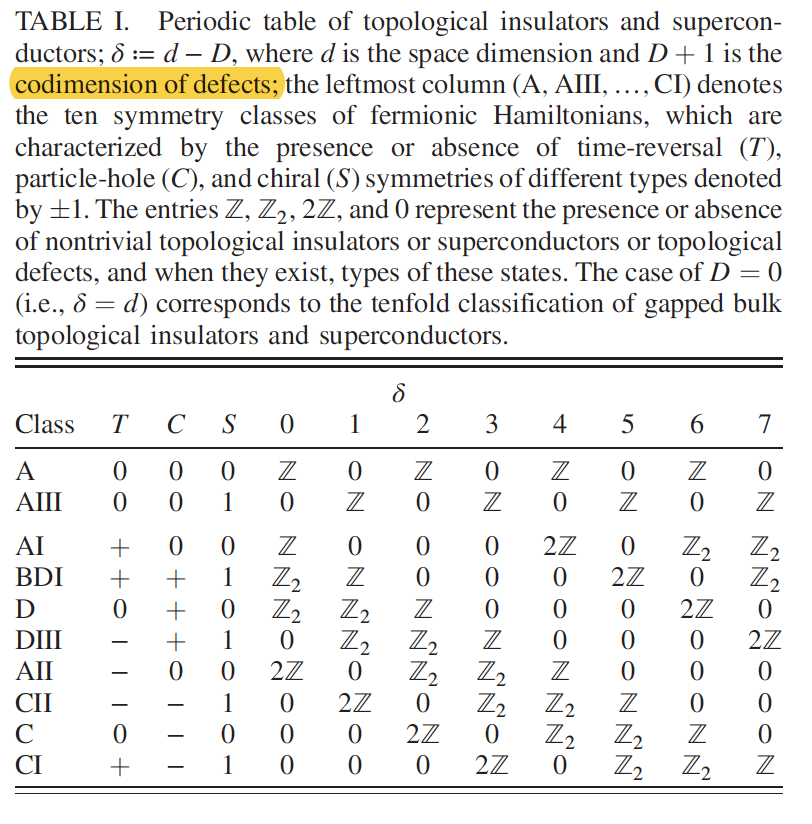
\includegraphics[height=10cm]{figures/tenfold.png}
\caption{Symmetry classes of the tenfold way}\label{fig:tenfold}
\end{center}
\end{figure}

\section{fully gapped free-fermion system and topological defects}
free fermion system is discribed by quadratic Bloch-BdG Hamiltonians:
\[\hat{H}=\sum_{r,r'}\hat{\Psi}_i^\dagger(r)H^{ij}(r,r')\hat{\Psi}_j(r')\]
and when asuming that $H(r,r')=H(r-r')$  we can make  fourier transformation and get $H(k)$.\par
we use the below hamitonian to discrib topological defects:
\[H_r(k)=H(k,r)\]
where the r is a parameter slowly modulate the Hamitonian and it includes spatial coordinates and/or a temporal parameter.Different defect Hamiltonians are distinguished by (i) the
AZ symmetry class s, (ii) the bulk dimension d, and (iii) the
defect codimension dc defined in terms of the dimension of
the defect $d_{defect}$ by
 \[d_c=d-d_{defect}\]
and we defined other parameters:
\[D=d_c-1\]
\[\delta=d-D\]
the ten symmetry classes can be divided to real AZ symmetry and complex AZ symmetry (where is no exisit of TRS PHS).for the eight real AZ symmetry ,it was shown that the classification of topological defects depends only on a single number
\[s-\delta=s-d+D ( mode 8)\]

\subsection{topological invariants}
the bloch wave function is defined in:
\[(k,r)\in BZ^d\times M^D\rightarrow S^{d+D}\]
\subsubsection{Primary series for s even: The Chern number}
For gapped topological phases and topological defects in
nonchiral classes (i.e., s is even), the Z-classified topologies
are characterized by the Chern number:
\[Ch_n=\frac{1}{n!}(\frac{i}{2\pi})^n\int_{BZ^d\times M^D}Tr(F^n)\]
where $n=\frac{d+D}{2}$ and F is the Berry Curvature:
\[F=dA+A^2\]
A is Berry Connection:
\[A^{\alpha \beta}(k,r)=\diracinner{u^{\alpha}}{du^{\beta}}\]

\clearpage

\part{Quantum Field Theory}
\setcounter{section}{0}
\section{The Klein-Golden Field}
\subsection{classical point of view}
for a real klein-Golden field the quantaty is listed below:
lagrangian density:
\[\mathcal{L}=\frac{1}{2}\dot{\phi}^2-\frac{1}{2}(\nabla\phi)^2-\frac{1}{2}m^2\phi^2=\frac{1}{2}\partial_{\mu}\phi\partial^{\mu}\phi-\frac{1}{2}m^2\phi^2\]
motion equation
\[(\partial^{\mu}\partial_{\mu}+m^2)\phi=0\]
Hamitonian density:
\[\mathcal{H}=\frac{1}{2}\pi^2+\frac{1}{2}(\nabla\phi)^2+\frac{1}{2}m^2\phi^2\]
\[\pi=\frac{\partial \mathcal{L}}{\partial\dot{\phi}}\]
using fourier transformation:
\[\phi(\vec{x},t)=\int \frac{d^3\vec{p}}{(2\pi)^3} e^{i\vec{p}\bullet\vec{x}}\phi(\vec{p},t)\]
the motion eqaution become:
\[\frac{\partial^2}{\partial t^2}+(|p|^2+m^2)=0\]
let $w_{\vec{p}}^2=|\vec{p}|^2+m^2$ one can get the motion eauation just like ocsillator:
\[\frac{\partial^2}{\partial t^2}+w_p^2=0\]

\subsection{quantilization of K-G Field}
\[[\phi(x),\pi(y)]=i\delta^{(3)}(x-y)\]
\[\phi(x)=\int \frac{d^3\vec{p}}{(2\pi)^3}\frac{1}{\sqrt{2\omega_p}}(a_p e^{ipx}+a_p^{\dagger}e^{-ipx})=\int \frac{d^3\vec{p}}{(2\pi)^3}\frac{1}{\sqrt{2\omega_p}}(a_p+a_{-p}^{\dagger})e^{ipx}\]
\[\pi(x)=\int \frac{d^3\vec{p}}{(2\pi)^3}(-i)\sqrt{\frac{\omega_p}{2}}(a_p e^{ipx}-a_p^{\dagger}e^{-ipx})=\int \frac{d^3\vec{p}}{(2\pi)^3}(-i)\sqrt{\frac{\omega_p}{2}}(a_p-a_{-p}^{\dagger})e^{ipx}\]
\[[a_p,a_{p'}^{\dagger}]=(2\pi)^3\delta^{(3)}(p-p')\]
to integrate the hamitonian densenty, we get the hamitonnian:
\[H=\int \mathcal{H}d^3x=\int \frac{d^3\vec{p}}{(2\pi)^3}w_p(a_p^{\dagger}a_p+\frac{1}{2}[a_p,a_p^{\dagger}])\]
to make a similar calculation, we get the monnmentum of the field:
\[P=-\int d^3x \pi(x)\nabla\phi(x)=\int\frac{d^3\vec{p}}{(2\pi)^3}pa_p^{\dagger}a_p\]
the state is defined as:
\[\diracr{p}=\sqrt{2E_p}a_p^{\dagger}\diracr{0}\]
and the interpratation of $\phi(x)\diracr{0}$ is that create a partical at position x.
and there are some realtions:
\[[H,a_p]=-a_pE_p\]
\[[H,a_p^{\dagger}]=a_p^{\dagger}E_p\]
\[\phi(x,t)=e^{iHt}\phi(x)e^{-iHt}=\int \frac{d^3\vec{p}}{(2\pi)^3}\frac{1}{\sqrt{2\omega_p}}(a_p e^{-ipx}+a_p^{\dagger}e^{ipx})|_{p_0=E_p}\]
\[\pi(x,t)=\frac{\partial}{\partial t}\phi(x,t)\]
we shold notice that the inner producr in the above relation is lorentz four vector's inner product.
\subsubsection{K-G Propagator}
\[D(x-y)=\diracl{0}\phi(x)\phi(y)\diracr{0}=\int \frac{d^3\vec{p}}{(2\pi)^3}\frac{1}{2E_p}e^{-ip(x-y)}\]
\[[\phi(x),\phi(y)]=D(x-y)-D(y-x)\]
the retared Green's Function:
\[D_R(x-y)=\theta(x_0-y_0)\diracl{0}[\phi(x),\phi(y)]\diracr{0}=\theta(x_0-y_0)\int \frac{d^3\vec{p}}{(2\pi)^3}\int \frac{dp_0}{2\pi i}\frac{-1}{p^2-m^2}e^{-ip(x-y)}\]
there we introduce a fomilism for delta function:
\[(\partial_t \delta(t))f(t)=-(\partial_t f(t))\delta(t)\]
the motion eauqtion of the retarded green function is :
\[(\partial^2+m^2)D_R(x-y)=-i\delta^{(4)}(x-y)\]
the fourier tranfer of the green function is:
\[D_R(p)=\frac{i}{p^2-m^2},D_R(x-y)=\int \frac{d^4p}{(2\pi)^4)}\frac{i}{p^2-m^2}e^{-ip(x-y)}\]
the feymann progatator for a klein-golden partial:
\[D_F(x-y)=\diracl{0}T\phi(x)\phi(y)\diracr{0}=\int \frac{d^4p}{(2\pi)^4)}\frac{i}{p^2-m^2+i\epsilon}e^{-ip(x-y)}\]



\section{The Dirac Field.}
the lagrangian:
\[\mathcal{L}=\bar{\Psi}(i\gamma^\mu\partial_\mu-m)\Psi\]
\subsection{representation of the lorentz group espically for 4 dimensions}
if we define 
\[J^{\mu,\nu}=i(x^{\mu}\partial^{\nu}-x^{\nu}\partial^{\mu})\]
then the six operator generate the three boost and three rotation of the lorentz group.\par
\[[J^{\mu,\nu},J^{\rho,\sigma}]=i(g^{\nu \rho}J^{\mu \sigma}-g^{\mu \rho}J^{\nu \sigma}-g^{\nu \sigma}J^{\mu \rho}+g^{\mu \sigma}J^{\nu \rho})\]
to clearly see theis operators is the generator ,we can use them to form the lorentz transfer:
\[V\rightarrow V'=(I-\frac{iJ^{\mu\nu}}{2}w_{\mu,\nu})V\]
in the above description, the $w_{\mu,\nu}$is just elements a random metric w which describ a lorentz tranferomation.\par
dirac's trick for the representation of lorentz group for n dimension:\par
if $\gamma^{\mu}$ is the n dimension metrics satisfying the relation:
\[\{\gamma^{\mu},\gamma^{\nu}\}=2g^{\mu\nu}I\]
then the six metrics:
\[S^{\mu\nu}=\frac{i}{4}[\gamma^{\mu},\gamma^{\nu}]\]
is the generator of the lorentz group for n dimensional representation(to prove  this, we just need to show the commutation relations ).\par

\subsection{the dirac algebra}

the dirac $\gamma$ metrics:
\begin{equation}
\sigma^1=\left(
\begin{array}{cc}
0&1\\
1&0\\
\end{array}
\right)
\sigma^2=\left(
\begin{array}{cc}
0&-i\\
i&0\\
\end{array}
\right)
\sigma^3=\left(
\begin{array}{cc}
1&0\\
0&-1\\
\end{array}
\right)
\end{equation}


\begin{equation}
\gamma^0=\left(
\begin{array}{cc}
0&1\\
1&0\\
\end{array}
\right)
\gamma^i=\left(
\begin{array}{cc}
0&\sigma^i\\
-\sigma^i&0\\
\end{array}
\right)
\end{equation}

then use the dirac's trick and we get the generator of the lorentz group:
\begin{equation}
S^{0i}=-\frac{i}{2}\left(
\begin{array}{cc}
\sigma^i&0\\
0&-\sigma^i\\
\end{array}
\right)
S^{ij}=\frac{1}{2}\epsilon^{ijk}\left(
\begin{array}{cc}
\sigma^k&0\\
0&\sigma^k\\
\end{array}
\right)=\frac{1}{2}\epsilon^{ijk}\Sigma^k
\end{equation}

some properties of the generator:
\[[\gamma^{\mu},S^{\rho,\sigma}]=(J^{\rho\sigma})^\mu_\nu\gamma^\nu\]
\[\Lambda_{\frac{1}{2}}^{-1}\gamma^\mu\Lambda_{\frac{1}{2}}=\Lambda^\mu_\nu \gamma^\nu\]
\[\Lambda_{\frac{1}{2}}=exp({-\frac{i}{2}\omega_{\mu\nu}S^{\mu\nu}})\]
since the metrics $S^{\mu\nu}$ is not hermitian, so we should take care of it when related to corresponding calculations.\par
some properties of these metrics:
\[\sigma^2\vec{\sigma}^*=-\vec{\sigma}\sigma^2\]
\[(p\bullet\sigma)(p\bullet\bar{\sigma})=p^2\]
we define 4 vector :
\[\sigma^\mu=(1,\vec{\sigma}),\bar{\sigma}^\mu=(1,-\vec{\sigma})\]
then the gamma metrics have a unit form:
\begin{equation}
\gamma^\mu=\left(
\begin{array}{cc}
0&\sigma^\mu\\
\bar{\sigma}^\mu&0\\
\end{array}
\right)
\end{equation}
we can use sixteen constant metrics to form a basis for the 4-dimensional metrics space:
\[1,\gamma^\mu,\gamma^{\mu\nu}=\gamma^{[\mu}\gamma^{\nu]},\gamma^{[\mu}\gamma^{\nu}\gamma^{\rho]},\gamma^{[\mu}\gamma^{\nu}\gamma^{\rho}\gamma^{\sigma]}\]
and we can use $\gamma^5$to simply the expresion for the last 5 metrics:
\[\gamma^5=i\gamma^0\gamma^1\gamma^2\gamma^3=-\frac{i}{4!}\epsilon^{\mu\nu\rho\sigma}\gamma_\mu\gamma_\nu\gamma_\rho\gamma_\sigma\]
we can the clrearly see that:
\[\gamma^{[\mu}\gamma^{\nu}\gamma^{\rho}\gamma^{\sigma]}=-i\epsilon^{\mu\nu\rho\sigma}\gamma^5\]
\[\gamma^{[\mu}\gamma^{\nu}\gamma^{\rho]}=-i\epsilon^{\mu\nu\rho\sigma}\gamma_\sigma\gamma^5\]
the properties of the $gamma^5$:
\[(\gamma^5)^\dagger=\gamma^5\]
\[(\gamma^5)^2=1\]
\[\{\gamma^5,\gamma^\mu\}=0\]
\[[\gamma^5,S^{\mu\nu}]=0\]
in dirac's representaion, we have:
\begin{equation}
\gamma^5=\left(
\begin{array}{cc}
-1&0\\
0&1\\
\end{array}
\right)
\end{equation}
the standard choice of theses metrics:
\[1,\gamma^\mu,\sigma^{\mu\nu}=\frac{i}{2}[\gamma^\mu,\gamma^\nu],\gamma^\mu\gamma^5,\gamma^5\]
a property of the Pauli metrics:
\[(\sigma^\mu)_{\alpha\beta}(\sigma_\mu)_{\gamma\delta}=2\epsilon_{\alpha\gamma}\epsilon_{\beta\delta}\]
\[(\bar{\sigma}^\mu)_{\alpha\beta}(\bar{\sigma}_\mu)_{\gamma\delta}=2\epsilon_{\alpha\gamma}\epsilon_{\beta\delta}\]

\subsection{classic solution to dirac equation }
the weyl spinor:
\[i\bar{\sigma}\partial \Psi_L=0\]
\[i\sigma\partial\Psi_R=0\]
the solution to the dirac equation:
\[(i\gamma^{\mu}\partial_\mu-m)\Psi(x)=0\]
using fourier tranfer we get the solotion for positive frequency:
\[\Psi(x)=\int \frac{d^4p}{(2\pi)^4)}u(p)e^{-ipx}\rightarrow (p_\mu\gamma^\mu-m)u(p)=0\]
the solution is :
\begin{equation}
u^s(p)=\left(
\begin{array}{c}
\sqrt{p\bullet\sigma}\xi^s\\
\sqrt{p\bullet\bar{\sigma}}\xi^s\\
\end{array}
\right)
\end{equation}
and the normalization is :
\[\bar{u}^ru^s=2m\delta^{r,s}\rightarrow (u^r)^{\dagger}u^s=2E_p\delta^{r,s}\]
the helicity operator:
\[\hat{h}=\hat{p}\bullet S=\frac{1}{2}\hat{p_i}\left(
\begin{array}{cc}
\sigma^i&0\\
0&\sigma^i\\
\end{array}
\right)
\]
using fourier tranfer we get the solotion for negetive frequency:
\[\Psi(x)=\int \frac{d^4p}{(2\pi)^4)}v(p)e^{ipx}\rightarrow (p_\mu\gamma^\mu+m)v(p)=0\]
the solution is :
\begin{equation}
v^s(p)=\left(
\begin{array}{c}
\sqrt{p\bullet\sigma}\eta^s\\
-\sqrt{p\bullet\bar{\sigma}}\eta^s\\
\end{array}
\right)
\end{equation}
and the normalization is :
\[\bar{v}^rv^s=-2m\delta^{r,s}\rightarrow (v^r)^{\dagger}v^s=2E_p\delta^{r,s}\]
\[\sum_s \bar{u}^s(p)u^s(p)=\gamma\bullet p+m\]
\[\sum_s \bar{v}^s(p)v^s(p)=\gamma\bullet p-m\]

\subsection{quantilization of the dirac field}
\[\mathcal{L}=\bar{\Psi}(i\gamma^\mu\partial_\mu-m)\Psi\]
\[H=\int d^3x\bar{\Psi}(-i\gamma\bullet \nabla+m)\Psi=\int d^3x\Psi^\dagger(-i\gamma_0\gamma\bullet \nabla+m\gamma_0)\Psi\]
the quantilized dirac field is:
\[\Psi(x)=\int \frac{d^3p}{(2\pi)^3}\frac{1}{\sqrt{2E_p}}\sum_s(a_p^su^s(p)e^{-ipx}+(b_p^s)^\dagger v^s(p)e^{ipx})\]
the anticommutation relations are:
\[\{a_p^r,(a_q^s)^\dagger\}=\{b_p^r,(b_q^s)^\dagger\}=(2\pi)^3\delta^3(p-q)\delta^{rs}\]
\[\{\Psi_a(x),\Psi_b^\dagger(y)\}=\delta^3(x-y)\delta_{ab}\]
then the hamitonian is :
\[H=\int \frac{d^3p}{(2\pi)^3}\sum_sE_p((a_p^s)^\dagger a_p^s+(b_p^s)^\dagger b_p^s)\]
the total monmentum operator is:
\[P=\int \frac{d^3p}{(2\pi)^3}\sum_s p((a_p^s)^\dagger a_p^s+(b_p^s)^\dagger b_p^s)\]
the angle monmentum is :
\[J=\int d^3x\Psi^\dagger(\vec{x}\times(-i\nabla)+\frac{1}{2}\Sigma)\Psi\]
the total charge:
\[Q=\int \frac{d^3p}{(2\pi)^3}\sum_s ((a_p^s)^\dagger a_p^s-(b_p^s)^\dagger b_p^s)\]
\subsubsection{the feyman propagator for dirac field}
the retared green function:
\[S_R(x-y)=(i\slashed{\partial}_x+m)D_R(x-y)\]
the greenn function satisfy the equation:
\[(i\slashed{\partial}_x-m)S_R(x-y)=i\delta^4(x-y)I\]
the fourier transform of  the retarded green function is:
\[S_R(p)=\frac{i(\slashed{p}+m)}{p^2-m^2}\]
the feymann propagator:
\[S_F(x-y)=\int \frac{d^4p}{(2\pi)^4}\frac{i(\slashed{p}+m)}{p^2-m^2+i\epsilon}e^{-i(x-y)}\]
\[S_F(p)=\frac{i(\slashed{p}+m)}{p^2-m^2+i\epsilon}\]

\subsection{discrete symmetrics in dirac field}
\textcolor{blue}{parity P,time reversal T,and chage interchage C}\par
1.Parity P:reverse the momentum but preserve the spin:
\[a_p^{s^\dagger}\diracr{0}\stackrel{P}{\longrightarrow}a_{-p}^{s^\dagger}\diracr{0}\]
\[Pa_p^sP=\eta_a a_{-p}^s\]
\[Pb_p^sP=\eta_b b_{-p}^s\]
\[\eta_a\eta_b=-1\]
\[P\Psi(t,x)P=\eta_a\gamma^0\Psi(t,-x)\]
\[P\bar{\Psi(t,x)}P=\eta_a^*\bar{\Psi(t,-x)}\gamma^0\]
2.Time Reversal T:reverse the momentum and spin\par
time reversal operator also act on the c-number:
\[T(c)=c^*T\]
define two vector operator:
\[a_p^s==(a_p^2,-a_p^1),b_p^s==(b_p^2,-b_p^1)\]
then time reversal operator T has the property:
\[Ta_p^sT=a_{-p}^{-s},Tb_p^sT=b_{-p}^{-s}\]
\[T\Psi(t,x)T=-\gamma^1\gamma^3\Psi(-t,x)\]
\[T\bar{\Psi}(t,x)T=\bar{\Psi}(-t,x)\gamma^1\gamma^3\]

3.charge conjugation C\par
\[Ca_p^sC=b_p^s,Cb_p^sC=a_p^s\]
\[C\Psi(x)C=-i(\bar{\Psi}\gamma^0\gamma^2)^{T}\]
\[C\bar{\Psi}C=(-i\gamma^0\gamma^2\Psi)^{T}\]



\section{The Vector Field}
Since the Largaran of the eletromagnetic field is:
\[\mathcal{L}=-\frac{1}{4}F^{\mu\nu}F_{\mu\nu}\]
so we can easily compute the quantity(which is myself defined):
\[\pi^{\mu\nu}=\frac{\partial L}{\partial (\partial_{\nu} A_\mu)}=F^{\mu\nu}\]
which implies the conjugate monmentum to $A_0$ is:
\[\pi^0=\frac{\partial L}{\partial (\partial_{0} A_0}=F^{00}=0\]
so the standard quantilization is not working here\par
to make a trick, we can use a new largrange:
\[\mathcal{L}=-\frac{1}{4}F^{\mu\nu}F_{\mu\nu}-\frac{\xi}{2}(\partial^\mu A_\mu)^2\]
which is the same as before in lorentz gauge:$\partial^\mu A_\mu=0$.\par
in such a form, the quantity as before defined is become:
\[\pi^{\mu\nu}=\frac{\partial L}{\partial (\partial_{\nu} A_\mu)}=F^{\mu\nu}-\xi\eta^{\mu\nu}(\partial^\sigma A_\sigma)\]
so at this time we have conjugate monmentum about the zero component:
\[\pi^0=\frac{\partial L}{\partial (\partial_{0} A_0})=-\xi\partial^\sigma A_\sigma=-\xi \partial\bullet A\]
from this formula ,it is clearly to see that if we want to quantelize the eletromagnetic field from the standard procedure ,the lorentz gauge is not working.\par
and the motion equation is :
\[\partial^2 A_\mu-(1-\xi)\partial_\mu(\partial\bullet A)=0\]
so when we choose $\xi=1$ which called the Feymann Gauge,the motion equation is just the same as the classic wavefunction:\par
\[A_\mu(x)=\int\frac{d^3 p}{(2\pi)^3}\frac{1}{\sqrt{2E_p}}\sum_{\lambda=0}^3(a_p^{(\lambda)}\epsilon_\mu^{(\lambda)}(p)e^{-ipx}+a_p^{(\lambda)\dagger}\epsilon_\mu^{(\lambda)*}(p)e^{ipx})\]
where symbol $\lambda$ denote the polarization of the photon.\par
\subsection{convention for the polarization vector}
first we have p fixed,and we randomly choose a unit vector n which satisfy $n^0>0$.at this time we have two vectors fixed.we choose vector $\epsilon^{(1),(2)}$ that in the plane which is vertical to the n and p and satisfying:
\[\epsilon^{\lambda}(p)\bullet \epsilon^{\lambda'*}(p)=-\delta_{\lambda,\lambda'} , with \lambda,\lambda'=1,2\]
we choose $\epsilon^3(p)$ in the plane which n and p located and make it vertical to n and is unit:
\[\epsilon^3(p)\bullet n=0, (\epsilon^3(p))^2=-1\]
to sommerize we have the relations in our convention:
\[\sum_{\lambda}\frac{\epsilon_\mu^\lambda(p)\epsilon_\nu^{\lambda *}(p)}{\epsilon^\lambda(p)\bullet\epsilon^{\lambda*}(p)}=\eta^{\mu\nu}\]
\[\epsilon^\lambda(p)\bullet\epsilon^{\lambda'*}(p)=\eta^{\lambda\lambda'}\]
and the quantilization relation is:
\[[A^\mu(x),\dot{A}^{\nu}]=-i\eta^{\mu\nu}\delta^3(x-y)\]

\section{Interacting fields and feymann diagrams}
a notation about the units:
\[\hbar=c=1\]
when using natural units,since:
\[E=mc^2=\hbar\nu=\frac{\hbar}{T}=\frac{\hbar c}{L}\]
so the quantity has these relations:
\[[E]=[M]=[T]^{-1}=[L]^{-1}\]
\subsection{Three Interacting System}
for the first interacting system,we consider the 4th-phi theory:
\[\mathcal{L}=\frac{1}{2}(\partial_\mu\phi)^2-\frac{1}{2}m^2\phi^2-\frac{\lambda}{4!}\phi^4\]
the second one is the quantum electrodynamics:
\[\mathcal{L}_{QED}=\mathcal{L}_{dirac} +\mathcal{L}_{maxwell}+\mathcal{L}_{in}=\bar{\Psi}(i\slashed{\partial}-m)\Psi-\frac{1}{4}(F_{\mu\nu})^2-e\bar{\Psi}\gamma^\mu\Psi A_\mu\]
and the last one is the Yukawa theory:
\[\mathcal{L}_{Yukawa}=\mathcal{L}_{dirac}+\mathcal{L}_{K-G}-g\bar{\Psi}\Psi\phi\]
\subsection{Wick's Theorem}
\[T\{\phi(x_1)\phi(x_2)\phi(x_3)\phi(x_4)\cdots\}=N\{\phi(x_1)\phi(x_2)\phi(x_3)\phi(x_4)\cdots+all-posibble-contractions\}\]
\subsection{cross section and S metrics}
we have the expression for the cross section in ananolous with S metrics is:
\[d\sigma=\frac{1}{2E_A2E_B|v_A-v_B|}(\prod\frac{d^3p_f}{(2\pi)^3}\frac{1}{2E_f})|M(p_A,p_B\rightarrow \{p_f\})|^2(2\pi)^4\delta^{(4)}(p_A+p_B-\sum p_f)\]
and the differential cross section is :
\[(\frac{d\sigma}{d\Omega})_{CM}=\frac{1}{2E_A2E_B|v_A-v_B|}\frac{|p_1|}{(2\pi)^24E_{cm}}|M(p_A,p_B\rightarrow \{p_f\})|^2\]
and the decay rate is:
\[d\Gamma=\frac{1}{2m_A}(\prod\frac{d^3p_f}{(2\pi)^3}\frac{1}{2E_f})|M(p_A,p_B\rightarrow \{p_f\})|^2(2\pi)^4\delta^{(4)}(p_A+p_B-\sum p_f)\]
where the M is associated with  the S metrics which is:
\[\hat{S}=\lim_{t\rightarrow \infty}e^{-i2\hat{H}t}\]
\[\hat{S}=1+i\hat{T}\]
\[(2\pi)^4\delta^{(4)}(p_A+p_B-\sum p_f)M(p_A,p_B\rightarrow \{p_f\})=\diracl{p_1,p_2\cdots} \hat{T}\diracr{p_Ap_B}\]
for the T operator ,we have the following formula to concuate it:
\[\diracl{p_1p_2\cdots p_n}i\hat{T}\diracr{p_Ap_B}=lim_{T\rightarrow\infty(1-i\epsilon)}({}_0\diracl{p_1p_2\cdots p_n}T({e^{-i\int_{-T}^TdtH_I(t)}})\diracr{p_Ap_B}_0)_{connected-and-amputated}\]

\section{Elementary process of quantum electrodynamics}
\subsection{Some useful relations}
\[(\bar{v}\gamma^\mu u)^*=\bar{u}\gamma^{\mu} v\]
any QED amplitute involving external fermions,when squared or summed over spin or overaged over spins, can be converted to trace of products of dirac metrics.for example for the process of figure \ref{fig:qedee} we have:\par
\begin{figure}
\begin{center}
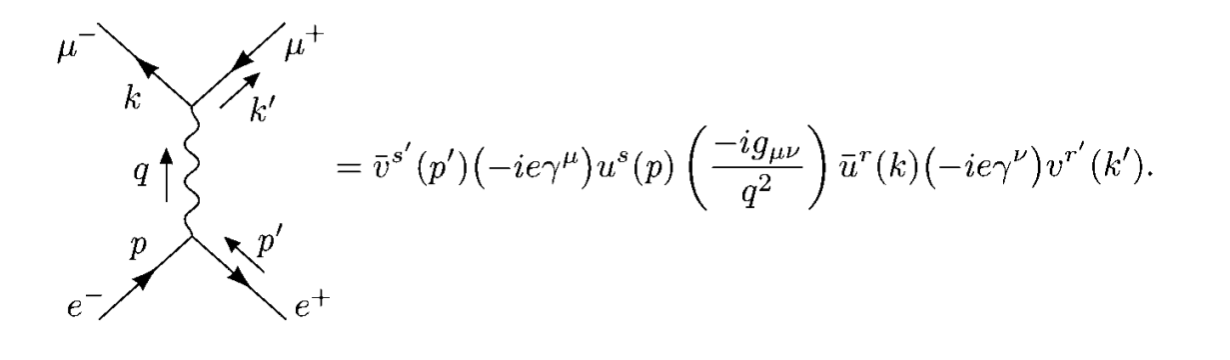
\includegraphics[height=5cm]{./figures/QEDee.PNG}
\caption{$e^+e^-\rightarrow \mu^+\mu^-$process}
\label{fig:qedee}
\end{center}
\end{figure}
\[\frac{1}{4}\sum_{spins}|\mathcal{M}|^2=\frac{e^4}{4q^4}trace[(\slashed{p'}-m_e)\gamma^\mu(\slashed{p'}+m_e)\gamma^\nu]trace[(\slashed{k}+m_\mu)\gamma_\mu(\slashed{k'}-m_\mu)\gamma_\nu]\]
the trace of an odd product of gamma metrics is zero(if n is odd):\par
\[trace[\gamma_1^{\mu}\cdots\gamma^{\mu'}_n]=0\]
\[tr[\gamma^\mu\gamma^\nu]=tr[2g^{\mu\nu}1-\gamma^\nu\gamma^\mu]\]
for the even number gamma metrics product ,we can anticommute the first one to the right and cycle it back ,we have the trace of two gamma metrics product:
\[tr[\gamma^\mu\gamma^\nu]=4g^{\mu\nu}\]
similarly for the four gamma metrics:\par
\[tr[\gamma^\mu\gamma^\nu\gamma^\rho\gamma^\sigma]=tr[2g^{\mu\nu}\gamma^\rho\gamma^\sigma-\gamma^\nu 2g^{\mu\rho}\gamma^\sigma+\gamma^\nu\gamma\rho 2g^{\mu\sigma}-\gamma^\nu\gamma^\rho\gamma^\sigma\gamma^\mu]\]
thus we have the following formula:
\[tr[\gamma^\mu\gamma^\nu\gamma^\rho\gamma^\sigma]=4(g^{\mu\nu}g^{\rho\sigma}-g^{\mu\rho}g^{\nu\sigma}+g^{\mu\sigma}g^{\nu\rho})\]
since $\gamma^5=i\gamma^0\gamma^1\gamma^2\gamma^3$,we have the trace fromula related to $\gamma^5$:
\[tr[\gamma^5]=0\]
\[tr[\gamma^\mu\gamma^\nu\gamma^5]=0\]
\[tr[\gamma^\mu\gamma^\nu\gamma^\rho\gamma^\sigma\gamma^5]=-4i\epsilon^{\mu\nu\rho\sigma}\]
and there are some formula for the antisymmetric tensor:
\[\epsilon^{\mu\nu\rho\sigma}\epsilon_{\mu\nu\rho\sigma}=-24\]
\[\epsilon^{\mu\nu\rho\sigma}\epsilon_{\mu\nu\rho\sigma'}=-6\delta^\sigma_{\sigma'}\]
\[\epsilon^{\alpha\beta\mu\nu}\epsilon_{\alpha\beta\rho\sigma}=-2(\delta^{\mu}_\rho\delta^\nu_\sigma-\delta^{\mu}_\sigma\delta^\nu_\rho)\]
and there is another useful formula:
\[tr[\gamma^\mu\gamma^\nu\gamma^\rho\gamma^\sigma\cdots]=tr[\cdots\gamma^\sigma\gamma^\rho\gamma^\nu\gamma^\mu]\]
if we set $C=\gamma^0\gamma^2$ then we have:
\[C^2=1\]
\[C\gamma^\mu C=-(\gamma^\mu)^T\]
when the gamma metrics is dotted inside the trace,one can always simplify it:
\[\gamma^\mu\gamma_\mu=g_{\mu\nu}\gamma^\mu\gamma^\nu=\frac{1}{2}g_{\mu\nu}\{\gamma^\mu,\gamma^\nu\}=g_{\mu\nu}g^{\mu\nu}=4\]
\[\gamma^\mu\gamma^\nu\gamma_\mu=-2\gamma^\nu\]
\[\gamma^\mu\gamma^\nu\gamma^\rho\gamma_\mu=4g^{\nu\rho}\]
\[\gamma^\mu\gamma^\nu\gamma^\rho\gamma^\sigma\gamma_\mu=-2\gamma^\sigma\gamma^\rho\gamma^\nu\]

\subsection{the unpolarized cross section for the process:$e^+e^-\rightarrow \mu^+\mu^-$}
when consider that $\frac{m_e}{m_{\mu}}$ is very small ,we can just set $m_e=0$,thus:
\[\frac{1}{4}\sum_{spins}|M|^2=\frac{8e^4}{q^4}[(p\bullet k)(p'\bullet k')+(p\bullet k')(p'\bullet k)+m_{\mu}^2(p\bullet p')]\]
after a long journey of calculation, we dervie the cross section for this process:
\[\frac{d\sigma}{d\Omega}=\frac{\alpha^2}{4E_{cm}^2}\sqrt{1-\frac{m_\mu ^2}{E^2}}[1+\frac{m_\mu ^2}{E^2}+(1-\frac{m_\mu ^2}{E^2})cos^2\theta]\]
and integrate it we can get the total cross section:
\[\sigma_{total}=\frac{4\pi \alpha^2}{3E_{cm}^2}\sqrt{1-\frac{m_\mu ^2}{E^2}}(1+\frac{1}{2}\frac{m_\mu ^2}{E^2})\]
we can define a unit of R:
\[R=\frac{4\pi \alpha^2}{3E_{cm}^2}\]
which means we regard  the cross section for the process $e^+e^-\rightarrow \mu^+\mu^-$ as a basic unit.\par

\subsection{$e^+e^-\rightarrow \mu^+\mu^-$:helicity structure}
\[\frac{d\sigma}{d\Omega}(e^-_Re^+_L\rightarrow \mu^-_L\mu^+_R)=\frac{\alpha^2}{4E_{cm}}(1+cos\theta)^2\]
\[\frac{d\sigma}{d\Omega}(e^-_Re^+_L\rightarrow \mu^-_R\mu^+_L)=\frac{\alpha^2}{4E_{cm}}(1-cos\theta)^2\]
\[\frac{d\sigma}{d\Omega}(e^-_Le^+_R\rightarrow \mu^-_L\mu^+_R)=\frac{\alpha^2}{4E_{cm}}(1-cos\theta)^2\]
\[\frac{d\sigma}{d\Omega}(e^-_Le^+_R\rightarrow \mu^-_R\mu^+_L)=\frac{\alpha^2}{4E_{cm}}(1+cos\theta)^2\]

for a right-hannded spinor ,we have:
\[\hat{p}\cdot\vec{\sigma}\eta=+\eta\]
for a left-handed spinor,we have:
\[\hat{p}\cdot\vec{\sigma}\eta=-\eta\]

some notes onn the bound state:
\[\sigma(e^+e^-\rightarrow B)=4\pi^2\frac{3\Gamma(B\rightarrow e^+e^-)}{M}\delta(E_{cm}^2-M^2)\]
the cross section for $e^+e^-$ to a bound state with spin-1 is that:
\[\sigma(e^+e^-\rightarrow B)=64\pi^3\alpha^2\frac{|\Psi(0)|^2}{M^3}\delta(E_{cm}^2-M^2)\]
and the decay rate  for the bound state is:
\[\Gamma(B\rightarrow e^+e^-)=\frac{16\pi\alpha^2}{3}\frac{|\Psi(0)|^2}{M^2}\]
\subsection{$e^-\mu^-\rightarrow e^-\mu^- $scatter}
the process's feymann diagram is presentend in figure \ref{fig:qedemu}.
\begin{figure}
\begin{center}
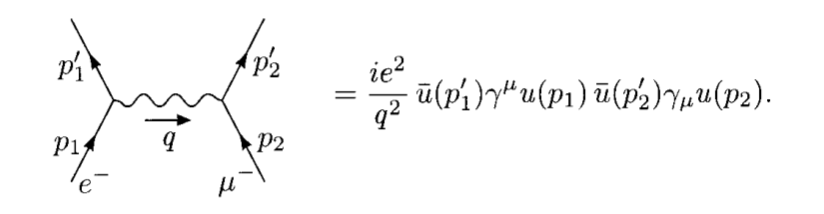
\includegraphics[height=5cm]{./figures/QEDemu.PNG}
\caption{$e^-\mu^-\rightarrow e^-\mu^-$process}
\label{fig:qedemu}
\end{center}
\end{figure}
just similar to the calculation with $e^+e^-\rightarrow \mu^+\mu^-$,we can easily get the deferiential cross section:
\[\frac{d\sigma}{d\Omega}=\frac{\alpha^2}{2k^2(E+k)^2(1-cos\theta)^2}[(E+k)^2+(E+kcos\theta)^2-m_{\mu}^2(1-cos\theta)]\]
Crossing Symmetry:
\[M(\phi(p)+\cdots\rightarrow\cdots)=M(\cdots\rightarrow \cdots\bar{\phi}(k))\]
where $\bar{phi}$ is the antipartical of $\phi$ and k=-p\par
Mandelstam Variable:
when the initial and final state are all two particals we can define the variables called Mandelstam Variable as below(see figure \ref{fig:man} for the process):
\begin{figure}
\begin{center}
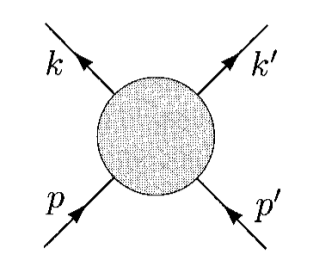
\includegraphics[height=5cm]{./figures/mandelstam.PNG}
\caption{illustration for the definition of mandelstam variable which involving 2-body to 2-body scattering process}
\label{fig:man}
\end{center}
\end{figure}
\[s=(p+p')^2=(k+k')^2\]
\[t=(k-p)^2=(k'-p')^2\]
\[u=(k'-p)^2=(k-p')^2\]
we can easily work out a relation:
\[s+t+u=\sum_i m_i^2\]

\subsection{Compton Scattering}
the feymann diagram for this process is presented in figure \ref{fig:compton}\par
\begin{figure}
\begin{center}
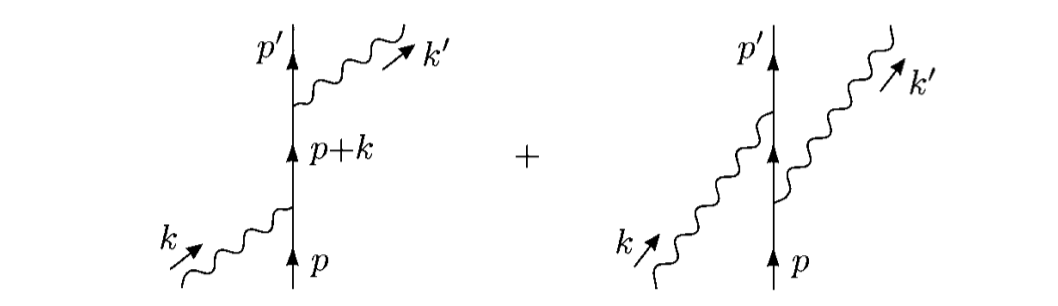
\includegraphics[height=5cm]{./figures/compton.PNG}
\caption{compton scattering process}
\label{fig:compton}
\end{center}
\end{figure}
so the amplitute is :
\[i\mathcal{M}=-ie^2\epsilon^*_\mu(k')\epsilon_\nu(k)\bar{u}(p')[\frac{\gamma^\mu\slashed{k}\gamma^\nu+2\gamma^{\mu}p^\nu}{2p\bullet k}+\frac{-\gamma^\nu\slashed{k'}\gamma^\mu+2\gamma^\nu p^\mu}{-2p\bullet k'}]u(p)\]

similar to the sum of electron polarization,there is also a good relation for sum of the photon polarization which is:
\[\sum_{polarization}\epsilon_\mu^*\epsilon_\nu\rightarrow -g_{\mu\nu}\]
with this in mind, we can easily get the quantity we want:
\[\frac{1}{4}\sum_{spins}|M|^2=\frac{e^4}{4}\{\frac{I}{(2p\bullet k)^2}+\frac{II}{(2p\bullet k)(2p\bullet k')}+\frac{III}{(2p\bullet k')(2p\bullet k)}+\frac{IIII}{(2p\bullet k')^2}\}\]

after a long journey of calculation we have the relations below:
\begin{align}
\notag I&=tr[(\slashed{p'}+m)(\gamma^\mu\slashed{k}\gamma^\nu+2\gamma^\mu p^\nu)(\slashed{p}+m)(\gamma_\nu\slashed{k}\gamma_\mu+2\gamma_\mu p_\nu)]\\
\notag&=16(4m^4-2m^2p\bullet p'+4m^2p\bullet k-2m^2p'\bullet k+2(p\bullet k)(p'\bullet k))\\
&=16(2m^4+m^2(s-m^2)-\frac{1}{2}(s-m^2)(u-m^2))
\end{align}
where the s,t,u is the Mandelstam Variables.\par
similarly we can work out the other three terms:
\begin{align}
IIII=16(2m^4+m^2(u-m^2)-\frac{1}{2}(s-m^2)(u-m^2))
\end{align}
\begin{align}
II=III=-8(4m^4+m^2(s-m^2)+m^2(u-m^2))
\end{align}
finally we have :
\[\frac{1}{4}\sum_{spins}|M|^2=2e^4[\frac{p\bullet k'}{p\bullet k}+\frac{p\bullet k}{p\bullet k'}+2m^2(\frac{1}{p\bullet k}-\frac{1}{p\bullet k'})+m^4(\frac{1}{p\bullet k}-\frac{1}{p\bullet k'})^2]\]
when we work in the fram of lab,we can make all the p,p',k,k'  illustrated as figure \ref{fig:compton2}. \par
\begin{figure}
\begin{center}
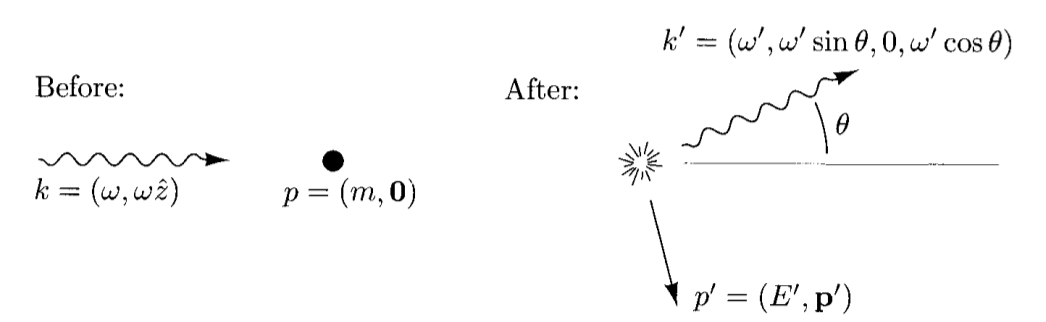
\includegraphics[height=5cm]{./figures/compton2.PNG}
\caption{compton scattering process in lab reference}
\label{fig:compton2}
\end{center}
\end{figure}
thus we have the differtial cross section:
\[\frac{d\sigma}{d(cos\theta)}=\frac{1}{2\omega}\frac{1}{2m}\frac{1}{8\pi}\frac{\omega'^2}{m\omega}(\frac{1}{4}\sum_{spins}|M|^2)\]
\[\frac{d\sigma}{d(cos\theta)}=\frac{\pi \alpha^2}{m^2}(\frac{\omega'}{\omega})^2[\frac{\omega'}{\omega}+\frac{\omega}{\omega'}-\sin ^2\theta]\]
where:
\[\omega'=\frac{\omega}{1+\frac{\omega}{m}(1-\cos\theta)}\]
this is called Klein-Nishina-Formula\par
when $\omega\rightarrow 0$,then $\frac{\omega'}{\omega}\rightarrow 0$,thus we have:
\[\frac{d\sigma}{d(cos\theta)}=\frac{\pi \alpha^2}{m^2}(1+\cos^2\theta)\]
which is the classical results which is known for all of us.\par




\section{Radiative Correlation}
\noindent Some Identities:\par
Ward Identity:
\[k_\mu M^{\mu}=0\]\par
Gordon Identity:
\[\bar{u}(p')\gamma^\mu u(p)=\bar{u}(p')\{\frac{p'^\mu+p^\mu}{2m}+\frac{i\sigma^{\mu\nu}q_\nu}{2m}\}u(p)\]
\subsection{Soft Bremsstrahlung}
The Current for a arbitory trajectory $y^\mu(\tau)$ is:
\[j^\mu(x)=e\int d\tau \frac{dy^\mu(\tau)}{d\tau}\delta^(4)(x-y(\tau))\]
we can consider a eletron with p get a sudden kick at$ (0,\vec{0})$ which illustrated in figure \ref{fig:soft}
\begin{figure}
\begin{center}
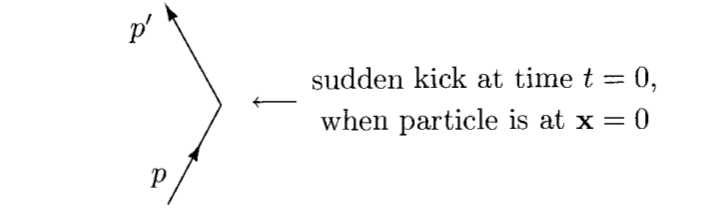
\includegraphics[height=4cm]{./figures/soft}
\caption{Soft Bremsstrahlung case: a electron get a sudden kick.}
\label{fig:soft}
\end{center}
\end{figure}
for this process, we can use the current as a source to solve the maxwell equation to get the potential:
\[A^{\mu}(x)=\int \frac{d^4k}{(2\pi)^4}e^{-ikx}\frac{-ie^2}{k^2}(\frac{p'^\mu}{p\bullet k'+i\epsilon}-\frac{p^\mu}{p\bullet k-i\epsilon})\]
and the riadiative part of the potential is:
\[A^\mu_rad(x)=Re\int \frac{d^3k}{(2\pi)^3}e^{-ikx}A^\mu(k)\]
where:
\[A^\mu(k)=\frac{-e}{|\vec{k}|}(\frac{p'^\mu}{p\bullet k'+i\epsilon}-\frac{p^\mu}{p\bullet k-i\epsilon})\]
and the energy radiatied is:
\[E=\int \frac{d^3k}{(2\pi)^3}\sum_{\lambda=1,2}\frac{e^2}{2}(\frac{2p\bullet p'}{(k\bullet p')(k\bullet p)}-\frac{m^2}{(k\bullet p')^2}-\frac{m^2}{(k\bullet p)^2})\]
Calculating the same quantity using quantum theory:
\[d\sigma(p\rightarrow p'+\gamma)=d\sigma(p\rightarrow p')\int \frac{d^3k}{(2\pi)^3}\frac{1}{2k}\sum_{\lambda=1,2}e^2|\epsilon_\lambda\bullet(\frac{p'}{p'\bullet k}-\frac{p}{p\bullet k})|^2\]
\[d\sigma(p\rightarrow p'+\gamma)=_{-q^2\rightarrow \infty}d\sigma(p\rightarrow p')\frac{\alpha}{\pi}\ln(\frac{-q^2}{\mu^2})\ln(\frac{-q^2}{m^2})\]
where $\mu$ is assumed tiny mass for photon to solve the divergence.\par
\subsection{The Electron Vetex Function}
Just as the figure \ref{fig:vertex} shows,we suppose the vertex is:
\[-ie\Gamma^\mu(p',p)\] 
\begin{figure}
\begin{center}
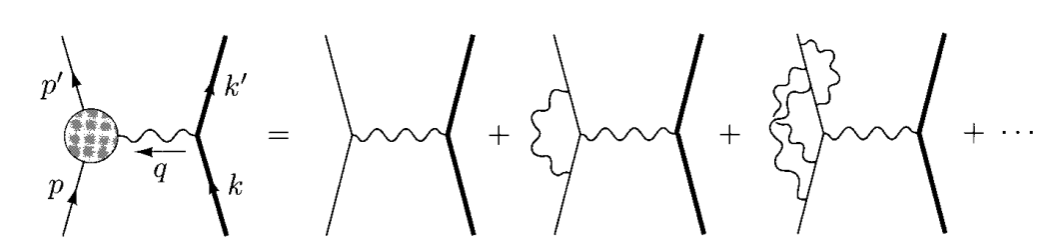
\includegraphics[height=4cm]{figures/vertex}
\caption{Electron Vertex Structure Illustration}
\label{fig:vertex}
\end{center}
\end{figure}
Using the Lorentz Invariance and Ward identity we can get the general form for it:
\[\Gamma^\mu(p',p)=\gamma^\mu F_1(q^2)+\frac{i\sigma^{\mu\nu}q_\nu}{2m}F_2(q^2)\]
where $F_1$ and $F_2$ is unkown function called \textcolor{red}{form factor}\par
for the Lande g-factor we have the ralation:
\[g=2(F_1(0)+F_2(0))\]
A trick for some integration:
\[\frac{1}{A_1A_2\cdots A_n}=\int_0^1dx_1\cdots dx_n\delta(\sum x_i-1)\frac{(n-1)!}{(x_1A_1+\cdots x_n A_n)^n}\]
\[\frac{1}{A_1^{m_1}A_1^{m_2}\cdots A_n^{m_n}}=\int_0^1dx_1\cdots dx_n\delta(\sum x_i-1)\frac{\prod x_i^{m_i-1}}{(\sum x_i A_i)^{\sum m_i}}\frac{\Gamma(m_1+\cdots m_n)}{\Gamma(m_1)\Gamma(m_2)\cdots\Gamma(m_n)}\]
\textcolor{red}{Feymann Parameter}:\par
\begin{align*}
\frac{1}{(k-p)^2(k^2-m^2)}&=\int_0^1 dxdy\delta(x+y-1)\frac{1}{[x(k-p)^2+y(k^2-m^2)]^2}\\
&=\int_0^1 dxdy\delta(x+y-1)\frac{1}{(k^2-2xk\cdot p+xp^2-ym^2)^2}
\end{align*}
when we define $l=k-xp$, then the whole integration is only rely on the $l^2$ and can trasfer to spherical coordinate to calculate the monmentum integration.the variable x,y is called Feymann Parameter.\par
we can use Wick rotation to change from Minkovski space to Eculid Space:
\[l^0=il_E^0;\hspace{3em} \vec{l}=\vec{l}_E\] 
then the intergration becomes:
\[\int d^4l\frac{1}{(l^2-\Delta)^m}=\frac{i}{(-1)^m}\frac{1}{(2\pi)^4}\int d^4l_E\frac{1}{(l_E^2+\Delta)^m}\]
the right hand side inner product of the above equation is the inner product in Eculid Space.
Using all the tricks above ,one can work out the diagram(figure \ref{fig:vertexcal}):
\begin{figure}
\begin{center}
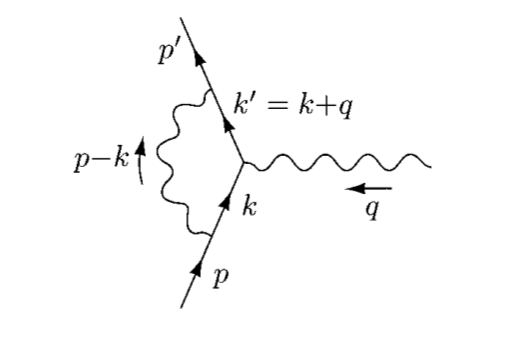
\includegraphics[height=4cm]{figures/vertexcal}
\caption{the order-$\alpha$ for $\Gamma^\mu$}
\label{fig:vertexcal}
\end{center}
\end{figure}
\begin{align*}
&\frac{\alpha}{2\pi}\int^1_0dxdydz\delta(x+y+z-1)\\
&\times \bar{u}(p')(\gamma^\mu[\ln\frac{z\Lambda^2}{\Delta}+\frac{1}{\Delta}((1-x)(1-y)q^2+(1-4z+z^2)m^2)]\\
&+\frac{i\sigma^{\mu\nu}q_\nu}{2m}[\frac{1}{\Delta}2m^2z(1-z)])u(p)
\end{align*}
where $\Lambda$ is a Parameter Introduced to solve the divergence.:
\[\frac{1}{(k-p^2)+i\epsilon}\rightarrow_{\Lambda\rightarrow \infty} \frac{1}{(k-p^2)+i\epsilon}-\frac{1}{(k-p^2)-\Lambda^2+i\epsilon}\]
with such substraction,the divergence of this type:
\[\int dl^2\frac{l^4}{(l^2+\Delta)^3}\rightarrow\int dl^2(\frac{l^4}{(l^2+\Delta)^3}-\frac{l^4}{(l^2+\Delta_\Lambda)^3})\]
\subsection{Summution And Interpreatation of Infrared Divergence.}
\begin{figure}
\begin{center}
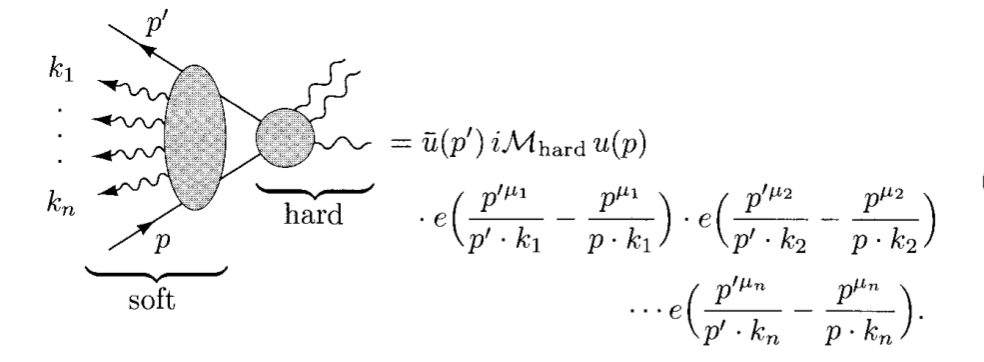
\includegraphics[height=4cm]{figures/VertexForm}
\caption{One can work out such diagram}
\end{center}
\end{figure}
and for a vitural photon such as the diagram like figure \ref{fig:vertexcal},Its value is(when connected to another diagram):
\[\frac{e^2}{2}\int \frac{d^4 k}{(2\pi)^4}\frac{-i}{k^2+i\epsilon}(\frac{p'}{p'\cdot k}-\frac{p}{p\cdot k})(\frac{p'}{-p'\cdot k}-\frac{p}{-p\cdot k})=X\]
with above calculation :
\[X=-\frac{\alpha}{2\pi}f_{IR}(q^2)\ln\frac{-q^2}{\mu^2}\]
\begin{figure}
\begin{center}
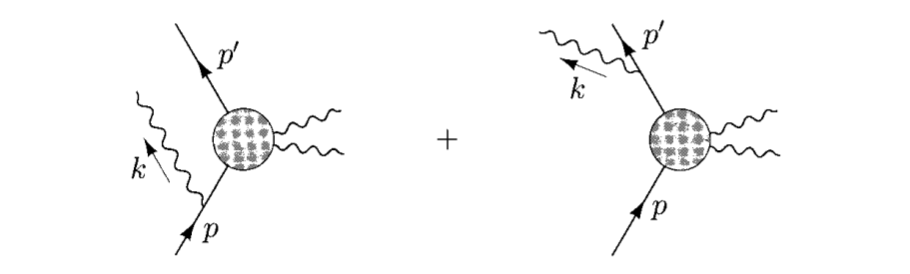
\includegraphics[height=4cm]{figures/realphoton}
\caption{scattering a real photon process}
\label{fig:realphoton}
\end{center}
\end{figure}
and the differential cross section for scattering a real photon like diagram(figure \ref{fig:realphoton}) is:
\[\int \frac{d^3k}{(2\pi)^3} \frac{1}{2k}(-g_{\mu\nu})(\frac{p'^\mu}{p'\cdot k}-\frac{p^\mu}{p\cdot k})(\frac{p'^\nu}{p'\cdot k}-\frac{p^\nu}{p\cdot k})=Y\]
with above calculation,we have:
\[Y=\frac{\alpha}{\pi}f_{IR}(q^2)\ln\frac{E_l^2}{\mu^2}\]
so we have:
\[\sum_{n=0}^\infty\frac{d\sigma}{d\Omega}(p\rightarrow p'+n\gamma)=\frac{d\sigma}{d\Omega}(p\rightarrow p')e^Y\]
and the correction for arbitrary vitural photon is:
\[\sum^{\infty}_{n=0}\frac{1}{n!}X^n=e^{X}\]
so the total differential cross section obseverd is:
\begin{align*}
(\frac{d\sigma}{d\Omega})_{measured}&=\frac{d\sigma}{d\Omega}(p\rightarrow p')e^{2X}e^Y\\
&=\frac{d\sigma}{d\Omega}(p\rightarrow p')e^{-\frac{\alpha}{\pi}f_{IR}(q^2)\ln\frac{-q^2}{E_l^2}}
\end{align*}
\par
\begin{center}
\textcolor{red}{\large{Which Is Not Depend On The  Vitural Photon Mass $\mu$}}
\end{center}


\section{Radiative Correlation:Some formal Development}
\subsection{Field Strength Renormalization}
we can use the spectrol of interacting hamitonian H to create a identity operator,since H is commute with the total momentum P,we can choose the states with:
\[\diracr{\Omega},\diracr{\lambda_0},\diracr{\lambda_p}\]
where the relations is:
\[H\diracr{\Omega}=0\diracr{\Omega},P\diracr{\Omega}=0\diracr{\Omega}\]
\[H\diracr{\lambda_0}=E_0\diracr{\lambda_0}=m_\lambda\diracr{\lambda_0},P\diracr{\lambda_0}=0\diracr{\lambda_0}\]
\[H\diracr{\lambda_p}=E_p\diracr{\lambda_p},P\diracr{\lambda_p}=p\diracr{\lambda_p}\]
where,
\[E_p=\sqrt{|\vec{p}|^2+m_\lambda^2}\]
since the state with total momentum zero is not only one,so different $\lambda$ give the different such states;\par
then we can use there states to construct the identity operotor:
\[1=\diracr{\Omega}\diracl{\Omega}+\sum_\lambda\int\frac{d^3p}{(2\pi)^3)}\frac{1}{2E_\lambda}\diracr{\lambda_p}\diracl{\lambda_p}\] 
insert this operotor into the correction function one can get:
\[\diracl{\Omega}\phi(x)\phi(y)\diracr{\Omega}=\sum_\lambda\int\frac{d^4p}{(2\pi)^4)}\frac{i}{p^2-m_\lambda^2+i\epsilon}|\diracl{\Omega}\phi(0)\diracr{\lambda_0}|^2\]
so we have dervied the Kallen-Lehmann spectral representation of the two-points function:
\[\diracl{\Omega}T\phi(x)\phi(y)\diracr{\Omega}=\int \frac{dM^2}{2\pi}\rho(M^2)D_F(x-y,M^2)\]
and the general form for $\rho(M^2)$ is:
\[\rho(M^2)=\sum_{\lambda} 2\pi\delta(M^2-m_\lambda^2)|\diracl{\Omega}\phi(0)\diracr{\lambda_0}|^2\]
\[\rho(M^2)=2\pi\delta(M^2-m_\lambda^2)Z+nothing-untill- M^2\gtrsim (2m)^2\]
we call Z as the \textcolor{red}{field strength renormalization}\par
and the fourier transfer of the two points function is:
\[\int d^4xe^{ipx}\diracl{\Omega}T\phi(x)\phi(0)\diracr{\Omega}=\frac{iZ}{p^2-m^2+i\epsilon}+\int_{\sim 4m^2}^\infty\frac{dM^2}{2\pi}\rho(M^2)\frac{i}{p^2-M^2+i\epsilon}\] 
and for the dirac firld,the quantity is:
\[\int d^4xe^{ipx}\diracl{\Omega}T\psi(x)\bar{\psi}(0)\diracr{\Omega}=\frac{iZ(\slashed{p}+m)}{p^2-m^2+i\epsilon}+\cdots\]
\subsection{The LSZ reduction formula}
Lehmann,Symanzik,Zimmerman;\par
\begin{align*}
&\prod_1^n\int d^4x_ie^{ip_ix_i}\prod_1^m\int d^4y_je^{-ik_jy_j}\diracl{\Omega}T\{\phi(x_1)\cdots\phi(x_n)\phi(y_1)\cdots\phi(y_m)\}\diracr{\Omega}\\
&\sim_{p_i^0\rightarrow +E_{\vec{p}_i},k_j^0\rightarrow +E_{\vec{k}_j}}=(\prod_1^n\frac{i\sqrt{Z}}{p_i^2-m^2+i\epsilon})(\prod_1^m\frac{i\sqrt{Z}}{k_j^2-m^2+i\epsilon})\diracl{p_1\cdots p_n}S\diracr{k_1\cdots k_m}
\end{align*}
using LSZ reduction formula,one can work out the feymann diagrammatic method for the  S metrics elements \ref{fig:amputa}
\begin{figure}
\begin{center}
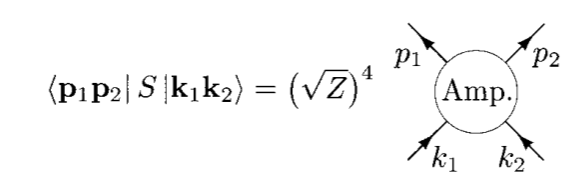
\includegraphics[height=4cm]{./figures/AmputatedFey}
\caption{Using LSZ formula to calculate the S metrics elements.}
\label{fig:amputa}
\end{center}
\end{figure}
\subsection{The Optical Theorem}
since 
\[S^{\dagger}S=1\]
on can get the result:
\[-i[T-T^{\dagger}]=T^{\dagger}T\]
insert a complete set of intermedia states one can get:
\begin{align*}
&-i[M(k_1k_2\rightarrow p_1p_2)-M^*(p_1p_2\rightarrow k_1k_2)]
\\
&=\sum_n(\prod_{i=1}^n\int \frac{d^3q_i}{(2\pi)^3}\frac{1}{2E_i})M^*(p_1p_2\rightarrow \{q_i\})M(k_1k_2\rightarrow\{q_i\})\times(2\pi)^4\delta^{(4)}(k_1+k_2-\sum_iq_i)
\end{align*}
so one can get the optical theorem:
\[2Im M(k_1k_2\rightarrow k_1k_2)=2E_{cm}p_{cm}\sigma_{tot}(k_1k_2\rightarrow anything)\]
\subsection{The Ward-Takahashi Identity}
the warden identity is illustated in figure \ref{fig:warden}.\par Ward identity is the diagrammatic expression of the current conservation,which is in turn a consequence of gauge invariance\par
\begin{figure}
\begin{center}
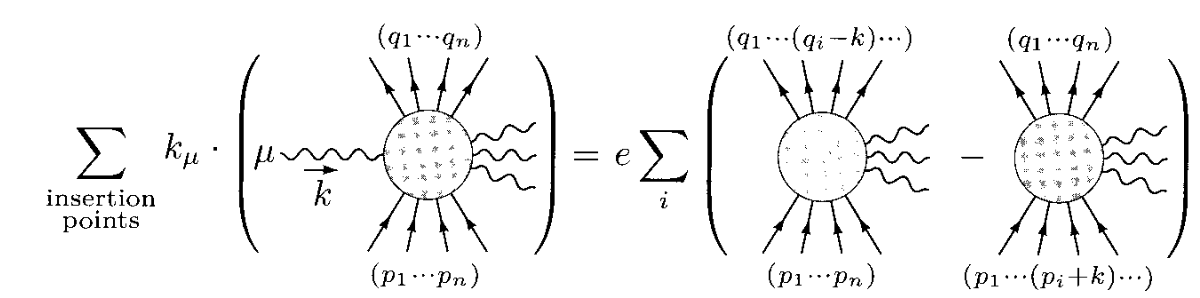
\includegraphics[height=4cm]{figures/warden}
\caption{The Ward-Takahashi Identity}
\label{fig:warden}
\end{center}
\end{figure}

\subsection{Renormalization of the Electric Charge}
the definition and diagram is illustrated as figure \ref{fig:loop1} and \ref{fug:loop2}。from the ward identity ,one can expect the form:\par
\begin{figure}
\begin{center}
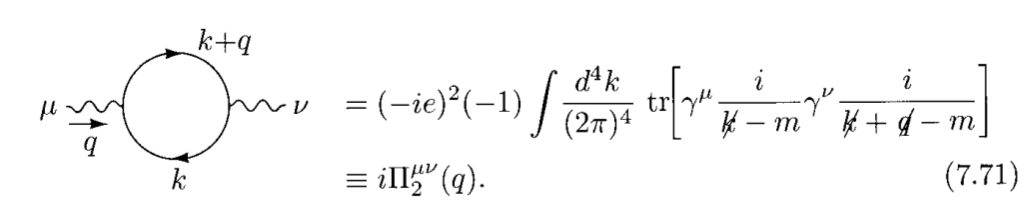
\includegraphics[height=3cm]{figures/loop1}
\caption{The feymann diagram for loop}
\label{fig:loop}
\end{center}
\end{figure}
\begin{figure}
\begin{center}
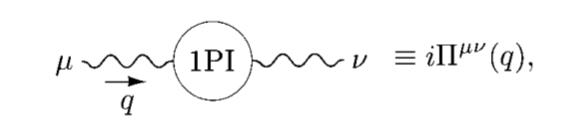
\includegraphics[height=3cm]{figures/loop2}
\caption{The 1PI Part}
\label{fig:loop2}
\end{center}
\end{figure}
\[\Pi^{\mu\nu}(q)=(q^2g^{\mu\nu}-q^\mu q^\nu)\Pi(q^2)\]
thus the calculation result is as the figure \ref{fig:loop3} shows.
\begin{figure}
\begin{center}
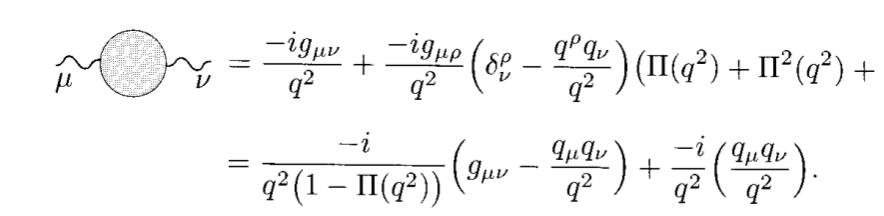
\includegraphics[height=3cm]{figures/loop3}
\caption{the result of the above digram}
\label{fig:loop3}
\end{center}
\end{figure}
\begin{figure}
\begin{center}
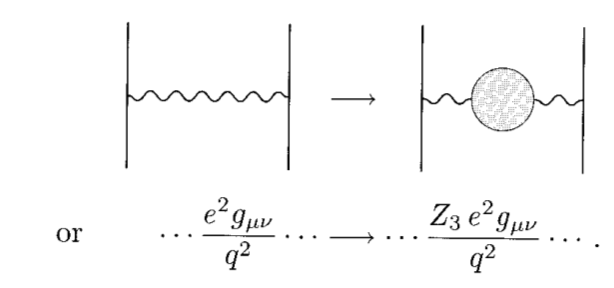
\includegraphics[height=5cm]{figures/loop4}
\caption{the charge regulization}
\label{fig:loop4}
\end{center}
\end{figure}
where the $Z_3$ is called charge regulization:
\[Z_3=\frac{1}{1-\Pi(0)}\]
\[e_0\rightarrow \sqrt{Z_3}e_0\]
after a long journey of calculation using feymann parameter, wick rotation ,one can work out:
\[i\Pi_2^{\mu\nu}(q^2)=-4ie^2\int _0^1dx\int\frac{d^4 l_E}{(2\pi)^4}\frac{\frac{1}{2}l_E^2g^{\mu\nu}-2x(1-x)q^\mu q^\nu+g^{\mu\nu}(m^2+x(1-x)q^2)}{(l_E^2+\Delta)^2}\]
with:
\[\Delta=m^2-x(1-x)q^2\]
which is baddly ultraviolet divergent. and voilate the ward identity.\par
\subsection{Dimennsional Regularization}
The area of a d dimensional unit sphere is:
\[\int d\Omega_d=\frac{2\pi^{\frac{d}{2}}}{\Gamma(\frac{d}{2})}\]
and one can work out the d-dimensional integration using gamma and beta function:
\[\int \frac{d^dl_E}{(2\pi)^d}\frac{1}{(l_E^2+\Delta)^2}=\frac{1}{(4\pi)^{\frac{d}{2}}}\frac{\Gamma(2-\frac{d}{2})}{\Gamma(2)}(\frac{1}{\Delta})^{2-\frac{d}{2}}\]
then we take the limit $d\rightarrow 4$ since:
\[\Gamma(2-\frac{d}{2})=\Gamma(2-\frac{4-\epsilon}{2})=\Gamma(\frac{\epsilon}{2})=\frac{2}{\epsilon}-\gamma+O(\epsilon)\]
then the above integration is:
\[\int \frac{d^dl_E}{(2\pi)^d}\frac{1}{(l_E^2+\Delta)^2}=_{d\rightarrow 4}=\frac{1}{(4\pi)^2}(\frac{2}{\epsilon}-\ln \Delta-\gamma+\ln(4\pi)+O(\epsilon))\]
similarly:
\[\int \frac{d^dl_E}{(2\pi)^d}\frac{1}{(l_E^2+\Delta)^n}=\frac{1}{(4\pi)^{\frac{d}{2}}}\frac{\Gamma(n-\frac{d}{2})}{\Gamma(n)}(\frac{1}{\Delta})^{n-\frac{d}{2}}\]
\[\int \frac{d^dl_E}{(2\pi)^d}\frac{l_E^2}{(l_E^2+\Delta)^n}=\frac{1}{(4\pi)^{\frac{d}{2}}}\frac{d}{2}\frac{\Gamma(n-\frac{d}{2}-1)}{\Gamma(n)}(\frac{1}{\Delta})^{n-\frac{d}{2}-1}\]
in d dimensional space:
\[g^{\mu\nu}g_{\nu\mu}=d\]
\[l^\mu l^\nu-\rightarrow \frac{1}{d}l^2g^{\mu\nu}\]
the dirac metric becomes a set of d metrics:
\[\{\gamma^\mu,\gamma^\nu\}=2g^{\mu\nu},tr[1]=4\]
\[\gamma^\mu\gamma^\nu\gamma_\mu=-(2-\epsilon)\gamma^\nu\]
\[\gamma^\mu\gamma^\nu\gamma^\rho\gamma_\mu=4g^{\nu\rho}-\epsilon\gamma^\nu\gamma^\rho\]
\[\gamma^\mu\gamma^\nu\gamma^\rho\gamma^\sigma\gamma_\mu=-2\gamma^\sigma\gamma^\rho\gamma^\nu+\epsilon \gamma^\nu\gamma^\rho\gamma^\sigma\]
after a long journey of calculation one can work out:
\[i\Pi_2^{\mu\nu}(q)=(q^2g^{\mu\nu}-q^\mu q^\nu)i\Pi_2(q^2)\]
with,
\[\Pi_2(q^2)=\frac{-8e^2}{(4\pi)^{\frac{d}{2}}}\int_0^1dx x(1-x)\frac{\Gamma(2-\frac{d}{2})}{\Delta^{2-\frac{d}{2}}}\]
\[\Pi_2(q^2)\sim_{d\rightarrow 4}=-\frac{2\alpha}{\pi}\int_0^1dx x(1-x)(\frac{2}{\epsilon}-\ln \Delta-\gamma+\ln(4\pi)+O(\epsilon))\]
\[V(r)=-\frac{\alpha}{r}(1+\frac{\alpha}{4\sqrt{\pi}}\frac{e^{-2mr}}{(mr)^{\frac{3}{2}}}+\cdots)\]
the rediative correction term is called Uehling Potential.\par


\section{Functional Method}
\subsection{Path Integrate in Quantum Mechanics}
\[U(q_a,q_b,T)=\diracl{q_a}e^{-iHT}\diracr{q_b}\]
when the hamitonian is weyl ordered we can express it of the form of integration in phase space:
\[U(q_a,q_b,T)=(\prod_i\int Dq(t)Dp(t))exp(i\int_0^Tdt\sum_i(p_i\dot{q_i}-H(q_i,p_i)))\]
for a scalor field:
\[U(q_a,q_b,T)=\int D\phi exp(i\int^T_{0}d^4x\mathcal{L}(\phi(x))\]
\subsection{functional quantization of scalor field}
The two-point correlation function is expressed as:
\[\diracl{\Omega}T\{\phi_H(x_1)\phi_H(x_2)\}\diracr{\Omega}=\frac{\int D\phi \phi(x_1)\phi(x_2)exp(i\int^T_{-T}d^4x\mathcal{L}(\phi(x)))}{\int D\phi exp(i\int^T_{-T}d^4x\mathcal{L}(\phi(x)))}\]
we can define a generating functional Z[J]:
\[Z[J]=\int D\phi e^{i\int d^4x(\mathcal{L}+J(x)\phi(x))}\]
one can work out this for free K-G theory:
\[Z[J]=Z_0e^{-\frac{1}{2}}\int d^4x d^4yJ(x)D_F(x-y)J(y)\]
then we can use this generating functional to get the correlation functions:
\[\diracl{\Omega}T\{\phi(x_1)\phi(x_2)\cdots\phi(x_n)\}\diracr{\Omega}=\frac{1}{Z[J]}(-i\frac{\delta}{\delta J(x_1)})(-i\frac{\delta}{\delta J(x_2)})\cdots(-i\frac{\delta}{\delta J(x_n)})Z[J]|_J=0\]
Z[J] is like the portion function in statistical physics,and J(x) is like the external field.\par
\subsection{functional quantization of EM field}
similarly,using the Faddeev and Popov trick,one can work out the correlation functions for EM Field:
\[\diracl{\Omega}TO(A)\diracr{\Omega}=lim_{T\rightarrow \infty(1-i\epsilon)}\frac{\int DA O(A)e^{i\int_{-T}^Td^4x[\mathcal{L}-\frac{1}{2\xi}(\partial^\mu A_\mu)^2]}}{\int DAe^{i\int_{-T}^Td^4x[\mathcal{L}-\frac{1}{2\xi}(\partial^\mu A_\mu)^2]}}\]
and the proton propogator is:
\[\frac{-i}{k^2+i\epsilon}(g^{\mu\nu}-(1-\xi)\frac{k^\mu k^\nu}{k^2})\]
\subsection{functional quantization of Dirac field}


\clearpage
\end{document}